\documentclass{article}
\usepackage{amsthm}
% \usepackage{ntheorem}
\usepackage{amsfonts}
\usepackage{graphicx}

% define break theorem style
\newtheoremstyle{break}
  {\topsep}{\topsep}%
  % {\itshape}{}%
  {\normalfont}{}%
  {\bfseries}{}%
  {\newline}{}%

% define definition 
\theoremstyle{break}
\newtheorem{definition}{Definition}[subsection]

\newcommand*{\Z}{\mathbb{Z}}
\newcommand*{\N}{\mathbb{N}}

\begin{document}
\title{Definitions for Abstract Algebra}
\author{Riley Weber}
\maketitle

Taken from \underline{Abstract Algebra: An Introduction} by Thomas W.
Hungerford (ISBN 978-1111569624). Created to study while taking MATH 3163:
Modern Algebra at UNC Charlotte. Definitions are ordered as they are in the
book and sectioned by chapter.

\section{Arithmetic in $\Z$ Revisited}
\subsection{}

\begin{definition}[Well-Ordering Axiom] 
  every non-empty subset of the set of non-negative integers has a least 
  element
\end{definition}

\subsection{}
\begin{definition}[Divisibility]
  Let $a, b \in \Z$ with $b \neq 0$. We say that $b$ divides $a$ and
  write $b \mid a$ if $a=bc$ for some $c \in \Z$.
\end{definition}

\begin{definition}[Greatest Common Divisor]
  Let $a, b \in \Z$, not both zero. The greatest common divisor ($gcd$) is
  the greatest integer that divides both $a$ and $b$. This means that if $d$ is
  the $gcd$ of $a$ and $b$, then
  \begin{enumerate}
    \item $d \mid a$ and $d \mid b$
    \item if $c \mid a$ and $c \mid b$, then $c \leq d$
  \end{enumerate}
  The greatest common divisor is often written $d = gcd(a,b)$ or simply
  $(a,b)$. it is also frequently called the greatest common \emph{denominator}.
\end{definition}

\subsection{}
\begin{definition}[Primality]
  An integer $p$ is said to be \textbf{prime} if $p \neq 0, \pm 1$ and the
  only divisors of $p$ are $\pm 1$ and $\pm p$.
\end{definition}

\section{Congruence in $\Z$ and Modular Arithmetic}
\subsection{}
\begin{definition}[Congruence Modulo $n$]
  Let $a, b, n \in \Z$ and $n > 0$. We say $a$ is congruent to $b$ modulo $n$
  and write $a \equiv b (mod n)$ if $n \mid a - b$.
\end{definition}

\begin{definition}[Congruence Class]
  Let $a, n \in \Z$ and $n > 0$. The congruence class of $a$ modulo $n$
  (written $[a]_n$ or $[a]$) is the set of all integers that are congruent to
  to $a$ modulo $n$. That is, $[a] = \{b | b \in \Z$ and $b \equiv a (mod n)\}$
\end{definition}

\begin{definition}[The Set of All Congruence Classes] 
  $\Z_n$, read "$\Z$ mod $n$" is the set of all congruence classes modulo n.
  Note that for every $n$ where $n \in \Z$ and $n > 1$, $\Z_n$ is a finite set,
  but each congruence class in that set is an infinite set. 
\end{definition}

\subsection{}
\begin{definition}[Addition and Multiplication in $\Z_n$]
  $[a] \oplus [b] = [a + b]$
  \\$[a] \odot [b] = [a \cdot b]$
\end{definition}

\subsection{}
\begin{definition}[Unit]
  Let $n \in \N$. A member of $\Z_n$ is a \textbf{unit} of $\Z_n$ if the
  equation $a \odot x = [1]$ has a solution in $\Z_n$.
\end{definition}

\pagebreak
\section{Rings}

\subsection{}

\begin{definition}[Ring]
  A ring is a nonempty set $R$ equipped with two operations (usually written as
  addition and multiplication) that satisfy the following axioms.

  For all $a, b, c \in R$:

  \renewcommand{\arraystretch}{1.5}
  \begin{tabular}{l p{6cm} p{4cm}}
    1. & If $a \in R$ and $b \in R$, then $a + b \in R$ & [Closure for
    addition] \\

    2. & $a + (b + c) = (a + b) + c$ & [Associative addition] \\

    3. & $a + b = b + a$ & [Commutative addition] \\

    4. & There is an element $0_R \in R$ such that $a + 0_R = a = 0_R + a$ for
    every $a \in R$ & [Additive identity or zero element] \\

    5. & For each $a \in R$, the equation $a+x=0_R$ has a solution in R &
    [Additive inverse] \\

    6. & If $a \in R$ and $b \in R$, then $ab \in R$ & [Closure for
    multiplication] \\

    7. & $a(bc) = (ab)c$ & [Associative multiplication] \\

    8. & $a(b + c) = ab + ac$ and $(a + b )c = ac + bc$ & [Distributive laws]
    \\
  \end{tabular}
\end{definition}

\begin{definition}[Commutative Ring]
  A commutative ring is a ring $R$ in which $ab = ba$ for all $a, b \in R$
  (commutative multiplication).
\end{definition}

\begin{definition}[Ring with Identity] A ring with identity is a ring $R$ that
  contains a special element $1_R$ such that $a \cdot 1_R = a = 1_R \cdot a$
  for all $a \in R$ (multiplicative identity).
\end{definition}

\begin{definition}[Integral Domains]
  An integral domain is a commutative ring $R$ with identity such that if $a, b
  \in R$ and $ab = 0_R$ then either $a = 0_R$ or $b = 0_R$.
\end{definition}

\begin{definition}[Field]
  A field is a commutative ring $R$ with identity $1_R$ such that if $a \in R
  \setminus \{0_R\}$ then $a$ is a unit (i.e. the equation $ax = 1_R$ has a
  solution in $R$)
\end{definition}

Following is a diagram which illustrates what common sets are also rings,
fields, and the like.

\begin{figure}
  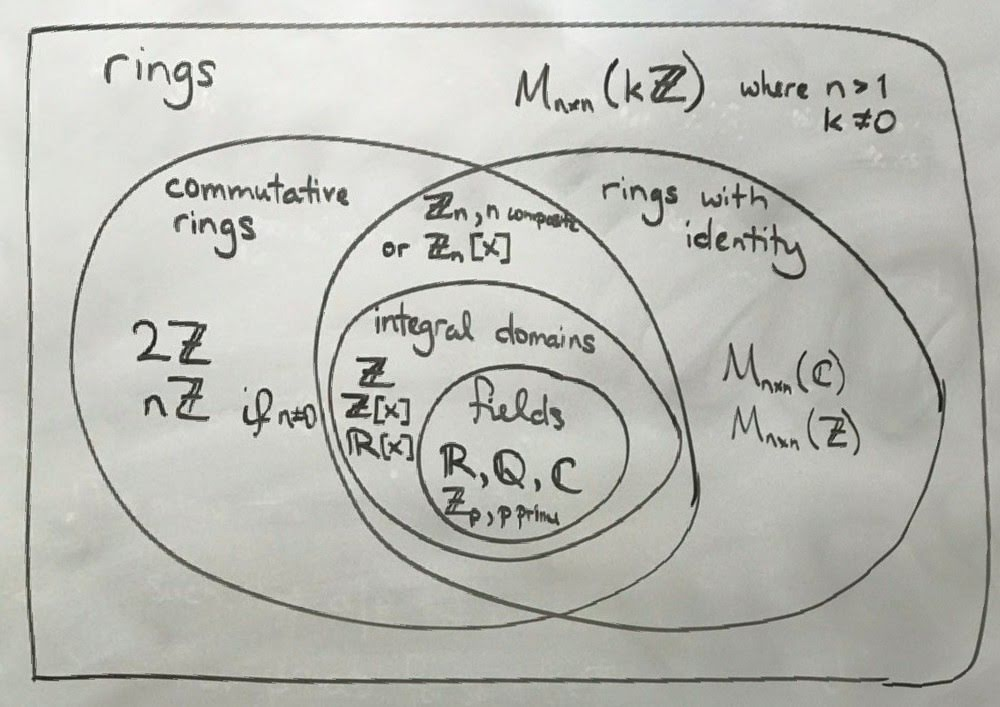
\includegraphics[width=\linewidth]{ring-venn-diagram.jpg}
\end{figure}

% \begin{definition}[]
% \end{definition}

\end{document}
